\documentclass{beamer}
\usetheme{Madrid}
\usepackage[spanish]{babel}
\usecolortheme{default}
\usepackage{emoji}
\usepackage[most]{tcolorbox}
\usepackage{listings}
\usepackage{xcolor}
\usepackage{colortbl}
\usepackage{graphicx}
\usepackage{algorithm}
\usepackage{algpseudocode}
\usepackage{float}
\usepackage{mathtools}
\usepackage{hyperref}
\makeatletter
\newcases{centercases}{\quad}
  {\hfil$\m@th\displaystyle{##}$\hfil}
  {$\m@th\displaystyle{##}$\hfil}{\lbrace}{.}
\makeatother

\usepackage{comment}
\usepackage{minted}

\usepackage{tikz}
\usetikzlibrary{arrows.meta,positioning}
\usetikzlibrary{calc}

% Define Python syntax highlighting
\lstdefinestyle{pythonstyle}{
    language=Python,
    basicstyle=\ttfamily\tiny,
    keywordstyle=\color{blue},
    commentstyle=\color{gray},
    stringstyle=\color{red},
    numbers=left,
    numberstyle=\tiny\color{gray},
    stepnumber=1,
    showstringspaces=false,
    frame=none,
    breaklines=true,
    numbersep=4pt, % Reduce space between numbers and text
    xleftmargin=10pt % Reduce left margin for compactness
}






%Information to be included in the title page:
\title[Infraestructura 
como Código] %optional
{Infraestructura 
como Código}

\subtitle{MISUM}

\author[José A.] % (optional, for multiple authors)
{José Antonio Hernández López\inst{1}}

\institute[UMU] % (optional)
{
  \inst{1}%
  Departamento de Informática y Sistemas\\
  Universidad de Murcia
}

%\date[VLC 2021] % (optional)
%{Very Large Conference, April 2021}



%\logo{\includegraphics[height=1cm]{overleaf-logo}}
\begin{document}

\frame{\titlepage}

\begin{frame}
\frametitle{Índice}
\tableofcontents
\end{frame}

\section{Infraestructura como código}

\begin{frame}{Infraestructura como código}

\begin{block}{Definición}
La infraestructura como código (IaC) utiliza un lenguaje de codificación descriptivo de alto nivel para automatizar el aprovisionamiento de la infraestructura informática
\end{block}

Esta automatización elimina la necesidad de que los desarrolladores aprovisionen y gestionen manualmente servidores, sistemas operativos, conexiones a bases de datos, ...

\begin{figure}
    \centering
    
\includegraphics[width=0.5\linewidth]{iac.png}
\end{figure}
    
\end{frame}


\begin{frame}{Infraestructura como código y DevOps}

\begin{itemize}
    \item Automatización total del despliegue: Evitas tareas repetitivas y manuales. La infraestructura se crea y configura con scripts o plantillas
    \item Ambientes reproducibles: La IaC asegura que los entornos (desarrollo, pruebas, producción) sean idénticos entre sí ya que las configuraciones están \textit{codificadas} 
    \item Velocidad y agilidad: Desplegar infraestructura ya no lleva horas/días... lleva minutos o segundos
    \item Control de versiones: La infraestructura está en Git igual que el código. Puedes hacer rollbacks si algo va mal
   
    
\end{itemize}
    
\end{frame}

\begin{frame}{Infraestructura como código y DevOps}

\begin{itemize}
     \item Mejora la colaboración Dev + Ops: Todo el equipo ve y entiende la infraestructura como parte del producto
    \item Seguridad mejor gestionada: Auditorías fáciles, todo está documentado y controlado. Permite aplicar políticas de seguridad mediante código (escanear los ficheros en busca malas prácticas antes del despliegue)
    \item Costes más bajos: Al automatizar, consumes solo lo que necesitas. Los entornos pueden crearse y destruirse bajo demanda, optimizando el uso de infraestructura
    
\end{itemize}
    
\end{frame}

\begin{frame}{Infraestructura como código: tipos de infraestructura}

Se distinguen dos tipos de infraestructuras:
\begin{itemize}
    \item Infraestructura mutable: es aquella que puede modificarse o actualizarse después de su aprovisionamiento original

    \textbf{Ejemplo}: servidor Linux de producción al que entras por SSH, actualizas software (e.g., Apache) y reinicias.

    \pause
    
    \item Infraestructura inmutable: no puede modificarse una vez que se aprovisiona originalmente.
    
    \textbf{Ejemplo}: si quieres actualizar una app en un contenedor (e.g., Docker), creas una nueva imagen y corres un nuevo contenedor.
\end{itemize}

\pause

\begin{block}{Tipo de infraestructura preferida en DevOps}
DevOps favorece la infraestructura inmutable ya que 

\begin{itemize}
    \item los entornos son 100\% reproducibles
    \item automatización completa CI/CD
\end{itemize}
\end{block}
    
\end{frame}

\begin{frame}{Infraestructura como código: enfoques}

Se distinguen dos tipos de enforque en IaC:

\begin{itemize}
    \item El \textbf{enfoque declarativo} describe el estado final deseado de la infraestructura, sin especificar cómo llegar a él

    \textbf{Ejemplos.} Terraform, Kubernetes Manifests, CloudFormation, etc.

    \pause
    
    
    \item El \textbf{enfoque imperativo} detalla los pasos y comandos específicos que deben ejecutarse en un orden determinado para lograr la configuración deseada

     \textbf{Ejemplos.} \textbf{Ansible}, Chef, Puppet (aunque tiene rasgos declarativos, depende del uso), etc.
\end{itemize}

\pause

\begin{block}{Tipo de enfoque preferido en DevOps}
En DevOps se suele usar una combinación de ambos:

\begin{itemize}
    \item Declarativa para la infraestructura: redes, MVs, clusters, etc
    \item Imperativa para configuración dentro del sistema: instalar paquetes dentro de VMs, crear usuarios y permisos, scripts de despliegue, etc.
\end{itemize}

\textbf{Ejemplo}: Un combo muy usado en la práctica es terraform + ansible.
\end{block}

\end{frame}

\section{GitOps}

\begin{frame}{GitOps}

\begin{block}{GitOps}

GitOps es una metodología de DevOps que usa Git como única fuente de verdad para gestionar y desplegar infraestructura y aplicaciones.

Todo lo que define el sistema (infraestructura + configuración + despliegues) se almacena en Git, y cualquier cambio se hace a través de pull requests o commits.

\end{block}

\begin{itemize}
    \item GitOps fue propuesto por Weaveworks en 2017 como una evolución natural de IaC.
    \item Objetivos: auditoría automática, revisión y control mediante Git y despliegues repetibles e inmutables
\end{itemize}
    
\end{frame}

\begin{frame}{GitOps: ejemplo a alto nivel}
Una set-up común en GitOps es tener dos repositorios:
\begin{itemize}
    \item Repo de aplicación: código fuente (ej. servicio en Node.js), Dockerfile, pipeline que genera imágenes y publica contenedores
    \item Repo de configuración conectados a un \textbf{controlador GitOps}: por ejemplo, Manifiestos Kubernetes
    
\end{itemize}

\pause

Flujo común:

{\scriptsize
\begin{enumerate}
    \item Un desarrollador hace un cambio en el código y crea un \textit{Pull Request}.
    \item El \textit{Pipeline} de CI construye una nueva imagen (por ejemplo, \texttt{app:v2}) y la sube al \textit{container registry}.
    \item El \textit{Pipeline} de CI modifica en el repositorio de configuración la versión de la imagen a \texttt{app:v2} y realiza \texttt{commit/push}.
    \item El operador GitOps (Argo CD / Flux) detecta automáticamente el cambio en Git.
    \item Argo CD aplica los \textit{manifests} al clúster de Kubernetes.
    \item Kubernetes actualiza el despliegue realizando un \textit{rollout} automático.
    \item El operador GitOps verifica continuamente que lo que está desplegado coincide con lo declarado en Git.
\end{enumerate}}

\end{frame}


\section{Ansible}

\begin{frame}{Ansible}

\begin{block}{Ansible}
Ansible es una herramienta de automatización y gestión de la configuración:
\begin{itemize}
    \item Con Ansible podremos gestionar decenas, cientos o miles de sistemas de forma sencilla, y además desde cualquier lugar
    \item La configuración de Ansible es sencilla, sólo exige la instalación de Python en cada uno de los equipos a administrar
\end{itemize}
    
\end{block}

\begin{figure}
    \centering
    
\includegraphics[width=0.5\linewidth]{ansible.jpg}
\end{figure}

    
\end{frame}

\begin{frame}{Ansible: arquitectura}

\begin{itemize}
    \item Nodo de control: sistema con Ansible instalado en el que se pueden ejecutar comandos.
    \item Nodo gestionado: sistemas gestionados por Ansible. Requisitos mínimos: Linux + Python + SSH.
    
\end{itemize}

\begin{figure}
    \centering
    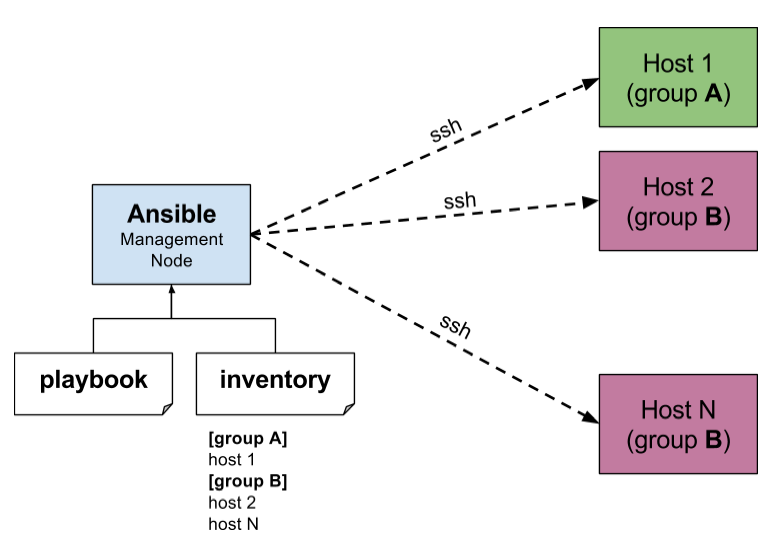
\includegraphics[width=0.5\linewidth]{ansible-ar.png}
\end{figure}
    
\end{frame}

\begin{frame}[fragile]{Ansible: inventarios}

El nodo de control tiene acceso a un inventario (llamado \texttt{hosts.ini}, \texttt{inventory.ini}, etc.). 

\begin{block}{Inventario}
El inventario es el archivo donde se definen los hosts (servidores) que Ansible gestionará, ordenados en grupos, y con variables asociadas si hace falta.
\end{block}

Ejemplo:

\begin{minted}[fontsize=\tiny]{yaml}
[web]
10.0.0.11
10.0.0.12

[db]
10.0.0.21
\end{minted}

\textbf{Nota.} En la instalación de Ansible se crea un archivo de configuración global (\texttt{/etc/ansible/hosts}) pero se suele generar uno dentro del proyecto.
    
\end{frame}

\begin{frame}[fragile]{Ansible: comandos ad hoc}

\begin{block}{Inventario}
Los comandos ad hoc en Ansible son comandos rápidos que se ejecutan sin necesidad de escribir un playbook.
\end{block}

\begin{itemize}
    \item Sirven para tareas puntuales como: probar la conexión, copiar archivos, reiniciar servicios, etc.
    \item Sintaxis:

    \begin{minted}[fontsize=\tiny]{bash}
ansible <hosts> -i <inventario> -m <módulo> -a "<argumentos>"
\end{minted}

\item Ejemplo: \texttt{ansible all -i inventory -m ping}

\item Un módulo es una unidad de acción en Ansible. Hay cientos (realmente miles) de módulos en Ansible.

\begin{itemize}
    \item apt: instalar paquetes en Debian/Ubuntu
    \item pip: gestión de paquetes en Python
    \item copy: copia archivos al host
    \item command: ejecuta comandos simples
    \item ...
\end{itemize}

\item Ejemplo: 

{\scriptsize\texttt{ansible webservers -m command -a ''/sbin/reboot -t now''}}
    
\end{itemize}

    
\end{frame}

\begin{frame}[fragile]{Ansible: playbooks}

\begin{block}{Playbook}
Un Playbook en Ansible es un archivo en formato YAML que contiene el plan completo de automatización:
qué hosts gestionar, qué tareas ejecutar y en qué orden.
\end{block}

Un playbook:

\begin{itemize}
    \item Se divide en un conjunto de plays.
    \item Cada play se dirige a un conjunto de hosts.
    \item Cada play tiene un conjunto de tareas.
    \item Cada tarea tiene un nombre y usa un módulo (con sus argumentos).
    \item Se ejecuta con \texttt{ansible-playbook -i inventario site.yml} donde \texttt{site.yml} es el playbook e \textit{inventario} es el inventario.
\end{itemize}



    
\end{frame}

\begin{frame}[fragile]{Ansible: playbooks}

\begin{minted}[fontsize=\tiny]{yaml}
---
# PLAY 1: Actualizar servidores web
- name: Actualizar y desplegar webserver
  hosts: web
  become: true
  tasks:
    - name: Instalar/Actualizar Nginx
      apt:
        name: nginx
        state: latest

    - name: Asegurar servicio Nginx iniciado
      service:
        name: nginx
        state: started
        enabled: true

# PLAY 2: Actualizar servidores de base de datos
- name: Actualizar y configurar DB
  hosts: db
  become: true
  tasks:
    - name: Instalar/Actualizar MariaDB
      apt:
        name: mariadb-server
        state: latest

    - name: Asegurar servicio DB iniciado
      service:
        name: mariadb
        state: started
        enabled: true
\end{minted}
    
\end{frame}

\begin{frame}[fragile]{Ansible: roles}

\begin{block}{Roles}
Los roles en Ansible son una forma estructurada y modular de organizar automatización.
\end{block}

Ejemplo:

\begin{minted}[fontsize=\tiny]{bash}
mi-proyecto/
├─ hosts.ini
├─ site.yml
└─ roles/
   ├─ webserver/
   │  └─ tasks/main.yml
   └─ dbserver/
      └─ tasks/main.yml
\end{minted}

En el \texttt{site.yml} (playbook principal):

\begin{minted}[fontsize=\tiny]{yaml}
- name: Configurar servidores web
  hosts: web
  become: true
  roles:
    - webserver

- name: Configurar servidores de base de datos
  hosts: db
  become: true
  roles:
    - dbserver
\end{minted}
\end{frame}

\begin{frame}[fragile]{Ansible: roles}

En \texttt{roles/dbserver/tasks/main.yml}:
\begin{minted}[fontsize=\tiny]{yaml}
- name: Instalar/Actualizar MariaDB
  apt:
    name: mariadb-server
    state: latest

- name: Asegurar que la DB está activa
  service:
    name: mariadb
    state: started
    enabled: true
\end{minted}

En \texttt{roles/webserver/tasks/main.yml}:
\begin{minted}[fontsize=\tiny]{yaml}
- name: Instalar/Actualizar Nginx
  apt:
    name: nginx
    state: latest

- name: Asegurar que Nginx está activo
  service:
    name: nginx
    state: started
    enabled: true
\end{minted}

    
\end{frame}

\begin{frame}{Ansible: Ansible Galaxy}

\begin{itemize}
    \item Los roles están muy bien para la reutilización. Sin embargo, es poco eficiente comenzar desde cero
    \item Ansible Galaxy, o simplemente ''Galaxy'', es un repositorio de contenido de Ansible aportado por la comunidad  (\url{https://galaxy.ansible.com/ui/})
    \item En Ansible Galaxy hay miles de roles disponibles para configurar y desplegar aplicaciones comunes.
\end{itemize}

\begin{figure}
    \centering
    
\includegraphics[width=0.2\linewidth]{cow.png}
\end{figure}
    
\end{frame}

\begin{frame}[fragile]{Ansible: Ansible Galaxy}

Por ejemplo:

\begin{enumerate}
    \item Ejecutamos \texttt{ansible-galaxy install geerlingguy.nginx}. Esto descarga el rol en \texttt{$\sim$/.ansible/roles/geerlingguy.nginx}.
    \item En nuestro playbook ya podemos referenciarlo:
    \begin{minted}[fontsize=\tiny]{yaml}
- hosts: web
  roles:
    - geerlingguy.nginx
\end{minted}

\end{enumerate}

\begin{figure}
    \centering
    
\includegraphics[width=0.2\linewidth]{cow.png}
\end{figure}

\end{frame}







\end{document}